\chapter{Physics-based Lidar Simulation - Transmitted Pulse}
A generic laser system consists of laser sources, optics, scanners(scanning lidar) or emitters(flash lidar), photon-detectors, timing devices, and a propagation medium as as air. The proposed physics-based full-system lidar simulator covers all the major components of a lidar system. 
%%%%%%%%%%%%%%%
%% 1. Laser Source
%%%%%%%%%%%%%%%

%% pulse model
\section{Transmitted pulse model}
In this work, the laser pulse is assumed to have a Gaussian distribution in time ~\citep{richmond2010direct,Budge2006SimulationLadarSIM}:
\begin{equation}  \label{eq:GauModel}
P_t(t) =\frac{E}{\sigma \sqrt{2\pi}}e^{-\frac{-t^2}{2\sigma^2}}
\end{equation}
where $E$ is the pulse energy of the laser, and $\sigma$ is the standard deviation of the Gaussian distribution. The relation between the standard deviation, the pulse width $\Delta t_w$ and the rise time $\Delta t_r$ are
\begin{equation} \label{eq:FWHM}
\Delta t_w=2\sigma\sqrt{2\ln2}\approx2.355\sigma
\end{equation}
\begin{equation} \label{eq:rt}
\Delta t_r\approx1.687\sigma
\end{equation}
assuming the area under the Gaussian curve is equal the area of a rectangular defined by the pulse width and the peak power. The derivation is given \todo{add appendix}. The peak power can be found as
\begin{equation} \label{eq:peakpower}
P_0 = \frac{E}{\Delta t_w} =\frac{E}{2\sigma\sqrt{2\ln2}}    
\end{equation}
Inserting Equation \eqref{eq:FWHM} and \eqref{eq:peakpower} to Equation \eqref{eq:GauModel}, the Gaussian pulse model used in this work is obtained
\begin{equation}\label{eq:pulsemodel}
P_t(t)=2\sqrt{\frac{\ln2}{\pi}}P_0e^{-4\ln2\frac{t^2}{\Delta t_w^2}}\approx0.94P_0e^{-4\ln2\frac{t^2}{\Delta t_w^2}}.
\end{equation}
Equation \eqref{eq:pulsemodel} also describes the relation between the height of the Gaussian pulse and the peak power: $h_{pulse}\approx0.94P_0$. Using Equation \eqref{eq:pulsemodel}, one can obtain the temporal power distribution of the transmitted pulse given the peak power, the pulse width of a laser source and a time sequence. The corresponding pulse energy, average power, and rise time can also be obtained using the equations above. However, one should note that a shortcoming of the model is that the model gives a non-zero signal power even for the time before the laser is fired ($t<0$), which causes a violation of causality.\todo{add pulse figure}

%% results and validation
\section{Results and Validation}
In this study, the parameter of the prototype lidar was utilized in the pulse model, and is given in \todo{chapter exp}. The pulse model was then validated by converting the modeled pulse in power to voltage and comparing with the start signal measured from the prototype lidar using an oscilloscope. The experimental setup for the validation is given in \todo{figure} and \todo{change number} 493 observations of the start signal were measured in voltage. The rise time, pulse width, and the height of the pulse generated by the pulse model and measured in the experiment were calculated. One example of the measured transmitted pulse is shown in Fig.~\ref{fig:pulse} along with the modeled pulse. The parameters of the laser were compared and shown in Table~\ref{table:param_pulseModel}. For the parameter of height of pulse, the bold value represent the original measured or modeled heights, while the other one is the corresponding value after the conversion between voltage and power.
\begin{figure}[htbp] % position options
\centering
\graphicspath{ {figures/} }
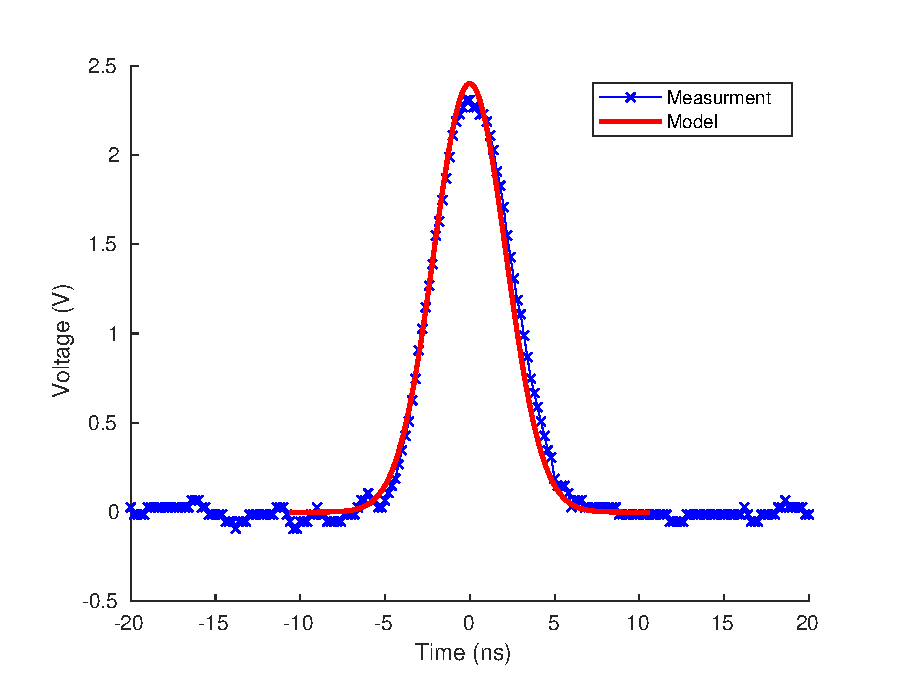
\includegraphics[width=0.8\textwidth]{figures/chapter4_pulse/Fig_pulse_model_meas.eps}
\caption{Example of pulse model}
\label{fig:pulse}
\end{figure}

\begin{table}[htbp]
\caption{{Parameters of Transmitted Pulse}}
\centering
\label{table:param_pulseModel}
\begin{tabular}{|l|l|l|l|}
\hline
Parameters    & Measurement & Model\\ \hline
Height of pulse (V) & $\mathbf{2.407\pm 0.107}$ &  $2.399$             \\ \hline
Height of pulse (W) & $558.04\pm 24.8$ &  $\mathbf{556.1}$             \\ \hline
Rise time (ns) & $3.119\pm0.413$ &  3.52   \\ \hline
Pulse width (ns) & $5.85 \pm0.318$ &  5  \\ \hline
\end{tabular}%
\end{table}

% sampling rate

% \subsection{Sampling rate}
% In the pulse model, we are using digital values to simulate continuous lase pulses, which requires a sufficient high sampling rate of the digital signal, so that (1) no aliasing occurs and the pulse shape is well represented, and (2) the natural of finite time intervals has minimum effects on the accuracy of distance measurements. However, on the other hand, if the sampling rate is too high, no additional information is provided and the computational cost is increased. Therefore, we studied the effect of different sampling rates on the distance measurement next and provide sduggestions on the selection of a proper sampling rate that balances the requirements and the computational cost.
\section{Sampling Rate}
1. in the previous result we have not talked about samplign rate. 
The sampling rate is another variable that needs to be considered, since
we use discret signal to simulate continous analog signal

wahab summaried the discussion of samplign rate of signal for chrom....and suggest (last sentense).
The response time or RC time constant is  an important factor for the sampling rate decision for lidar simualtion as well, in additino to other factors: timing device resoluion... 
Therefore, we listed the factors that need to be considered for the lidar simulation:

% 2. to be considered:
(1) represent signal well
-signal bw
(2) no effect on timing accuracy
(3) no effect on timing resolution
(4) represent noise and effect of noise on measurement well
-white noise ->  infinite high frequency, but the signal need to be process by a circuits => so we also have to consider prop delay
(5) computational cost

To decide a sampling rate for this study corresponding to the devic3 parameters, we performed tests on several different srs, and the check if the metris are meet. and chose the lowest one  meeting all the metrieis for lowest computational cost.
\subsection{Experiments}














% %%%%%%%%%%%%%%%
% %% Timing Module
% %%%%%%%%%%%%%%%

% \section{Time Discriminators}
% \subsection{Time-to-digital converter approaches}
% \subsection{Analog-to-digital converter approaches}

% \subsubsection{Digital version of the analog timing techniques}
% After an ADC converts analog signals to digital signals, different timing techniques are applied on a DSP to determine the time of the returning pulse. One approach is implementing a digital version of the analog timing techniques, i.e. leading-edge detection techniques or CFDs. The details of those methods are described in above sections and are skipped here, but it should be noticed that for the digital signals, the threshold generally does not coincide to the sample points of the signal. Therefore, interpolation between neighborhood samples is needed to find the exact time mark corresponding to the threshold value. Linear interpolation is a common selection, but the interpolation could affect the timing accuracy, depending on the local linearity of the signal. More specifically, if the curvature of a signal in the proximity of the threshold is large (the pulse has a nonlinear shape), time walk could occur. Note that this walk error is different than the walk error mentioned in the TDC-based approaches. The effect of the curvature is illustrated in Fig \textcolor{yellow}{(Fig10.27 Mahammad book). }

% \subsubsection{Detector and Estimator}
% The digital version of the analog timing techniques that utilize the ADC as a TDC limits the potential of the ADC, since the information contained in the digital signal is valuable for the improvement of the accuracy of signal detection and estimation. Therefore, time discrimination algorithms taking advantage of the shape information is illustrated next, which are generally composed of a detector and an estimator following a ADC. The function of the detector is to determine the presence or absence of a predefined signal from a signal contaminated by noise. In our case, if a Gaussian pulse with certain characteristics (\ie rise time, pulse width, \etc) is present in the returning signal. If the pulse is present, an estimator is needed to estimate the values of the parameters of the signal (arrival time of the pulse in our case) by mathematically modeling the signal. \\
% In this work, determining the presence of a pulse is performing a binary hypothesis test $\mathcal{H}_1$: pulse or $\mathcal{H}_0$: noise, and \cite{kay1998fundamentals} recommended using a Neyman-Pearson(NP) detector or Bayesian approaches for such a problem. Bayesian approaches require a prior knowledge of the likelihood of the hypotheses, or \emph{prior probabilities}: $P(\mathcal{H}_1)$ and $P(\mathcal{H}_0)$ , but it is usually not available for radar or lidar applications, neither for this work. Thus, the NP detector is considered in this study. The NP detector has been proven to be the optimal detector for radar/ laser signal detection\cite{kay1998fundamentals}, and has been widely utilized in many applications like target detection, medicine, nuclear energy, gravitational-wave astronomy, \etc\cite{Hoover2000LocatingResponse,Bousselham2007SamplingTiming,seto2001possibility,gronwall2007influence,gu2002detecting,Jordan2009RangeData,roman2000parametric,Ofek2017OptimalDetection,Vio2018MatchedImplementation}. In general, the NP detector conducts a likelihood ratio test(LRT\textcolor{yellow}{equation..}) for detection of a known deterministic pulse, \ie the pulse has no unknown parameters, while in our case some parameters of the pulses are unknown,\eg the arrival time (the amplitude of the pulse is less important). Therefore, a more general LRT(\emph{generalized likelihood ratio test}, or GLRT) is used for such situation, by using which the parameters of the pulse (arrival time) will be determined simultaneously. Consequently, our problem that the detecting the returning pulse and estimating the arrival time are combined to a single problem, and it can be solved by applying a NP detector with GLRT. The principle of the NP detector, LRT and GLRT will be introduced next followed by the application of the detection theories to solve our problem.

% \subsubsection{Neyman-Pearson Detector}
% \paragraph{Problem definition}
% First, we need to define our problem mathematically, that is,  to distinguish between the hypotheses $\mathcal{H}_1$: pulse or $\mathcal{H}_0$: noise:
% \begin{align}\label{eq: hy}
% \mathcal{H}_0:x[n]&=w[n]  &n=0, 1,\ldots, N-1\\
% \mathcal{H}_1:x[n]&=s[n-n_0]+w[n]  &n=0, 1,\ldots, N-1    
% \end{align}
% where $x$ is the returning digital signal,  $w$ is the noise following a Poisson distribution with the expected value $E[w]=W$, and $W$ is the mean of the total noise current which is the summation of the mean dark current $D$ and mean background current $B$, \ie $W = D + B$ , and $w\sim Pois(W)$. $s$ is our transmitted pulse that is deterministic and nonzero over the time interval $[0, M-1]$.  $n$ stands for each data point in the digital signal which is bounded by the observation time period $[0, N-1]$, and $n_0$ is the arrival time of the pulse, $n_0\in[0, N-M]$. Our goal is to decide the hypothesis a returning signal should fall with a certain false alarm rate $P_{fa}$, and if it is a pulse, we need to estimate the value of $n_0$.
% \paragraph*{Neyman-Pearson Theorem}
% The Neyman-Pearson theorem allows us to design a detector to achieve our goal: to maximize the detection probability $P_D$ for a given $P_{fa}  =\alpha$, decide $\mathcal{H}_1$ if the generalized likelihood ratio $L_G(x)$ is greater than a threshold $\gamma$; otherwise, decide $\mathcal{H}_0$: \textcolor{red}{need to talk about $\hat{n}_0$}
% \begin{equation} \label{eq:Lx}
% L_G(x)=\frac{p(x;\hat{n}_0,\mathcal{H}_1)}{p(x;\mathcal{H}_0)}\underset{\mathcal{H}_0}{\overset{\mathcal{H}_1}{\gtrless}}\gamma
% \end{equation}
% where the threshold $\gamma$ is found from
% \begin{equation}\label{eq:pfa}
% P_{fa}=\int_{\{x:L_G(x)>\gamma\}} p(x;\mathcal{H}_0)dx=\alpha
% \end{equation}
% And the detection probability $P_D$ is defined as
% \begin{equation} \label{eq:pd}
% P_D=\int_{\{x:L_G(x)>\gamma\}}p(x;\hat{n}_0, \mathcal{H}_1)dx
% \end{equation}
% The generalized likelihood ratio $L_G(x)$ indicates the likelihood of $\mathcal{H}_1$ versus the likelihood of $\mathcal{H}_0$, and the Equation \eqref{eq:Lx} is called the generalized likelihood ratio test (GLRT). The 'generalized' indicates the signal has unknown parameters. The probability density distribution (PDF) $p(x;\hat{n}_0,\mathcal{H}_1)$ stands for the PDF of the signal with an unknown parameter $\hat{n}_0$ under $\mathcal{H}_1$ hypothesis, and follows a Poisson distribution $Pois(S+W)$, where $S$ is the mean of the returning current. We also know that the PDF of the signal under hypothesis $\mathcal{H}_0$, $p(x;\mathcal{H}_0)\sim Pois(W)$. Given a Poisson random variable $x$ with the expected value $\lambda$ follows $Pois(x;\lambda) = \frac{e^{-\lambda}\lambda^X}{x!}$ after mathematical reorganization the GLRT is reduced to (The derivation of Equation \eqref{eq:Tx} is provided in \textcolor{yellow}{appendix}.):
% \begin{eqnarray} \label{eq:Tx}
% T(x) &=&\ln(L_G(x))=\sum_{n=\hat{n}_0}^{\hat{n}_0+M-1}x[n]k[n-\hat{n}_0] \underset{\mathcal{H}_0}{\overset{\mathcal{H}_1}{\gtrless}}\gamma'\\
% \gamma'&=&\ln\gamma+\sum_{n=0}^{M-1}s[n]\\
% k[n]&=&\ln(\frac{s[n]}{W}+1)
% \end{eqnarray}
% and Equation\eqref{eq:pfa} is changed to
% \begin{equation}\label{eq:pfa2}
% P_{fa}=Pr(T(x)>\gamma';\mathcal{H}_0)
% \end{equation}

% where $T(x)$ is the test statistic which is a function of our measurements, and $k$ is the template, which can be determined from the transmitted pulse. Equation\eqref{eq:Tx} indicates the GLRT calculates the cross-correlation of the signal $x[n]$ with the kernel for all possible $n_0$, and compare the maximum value that obtained when $n_0=\hat{n}_0$ with the threshold $\gamma'$. If the threshold is exceeded, a pulse is claimed to be present, and the arrival time is estimated as $\hat{n}_0$ (It will be proved in Section \ref{sec:MLE}). Otherwise, noise is claimed detected. Mathematically,\\
% \begin{align}
%     T(x)=\max_{n_0\in[0,N-M]}\sum_{n=\hat{n}_0}^{\hat{n}_0+M-1}x[n]k[n-n_0]\\
%     \hat{n}_0= \argmax_{n_0\in[0, N-M]}T(x)
% \end{align}
% % \begin{align}
% % T(x)=\max_{n_0\in[0,N-M]}\sum_{n=\hat{n}_0}^{\hat{n}_0+M-1}x[n]k[n-n_0]\\
% % \hat{n}_0= \argmax_{n_0\in[0, N-M]}T(x)
% % \end{align} 
% In practice, the $T(x)$ can be computed by using a detector to perform correlation with a predefined kernel, and such a detector is referred to as a \emph{correlator}. Alternatively, the $T(x)$ can also be obtained from the convolution of signal with the conjugated time-reversed of the kernel $k'[n]$, \ie for each timestamp $n$, the convolution result is
% \begin{align}\label{eq:mf}
% y[n]=\sum_{m=0}^nx[m]k'[n-m]\\
% k'[n]=s[N-1-n]
% \end{align}
% Equation\eqref{eq:mf} is known as a \emph{matched-filter}. The correlator and the matched-filter are proved mathematically equivalent, and the difference between the correlator and matched-filter is beyond the scope of this work and will not be discusses further. \textcolor{yellow}{Readers could refer to \cite{kay1998fundamentals} for details}.This work will focus on using Equation \eqref{eq:Tx} for illustration of the principle of the NP detector.\\
% Moreover, since the time complexity of convolution is $\mathcal{O}(MN)$($M$ and $N$ are the the number of points of the kernel and the signal), the correlation or convolution could be computational intensive if the signal contains a large number of data points. To accelerate the computation, the $T(x)$ can be implemented in the frequency domain by using Fast Fourier Transformation (FFT) of which the time complexity is $\hat{O}(N\log N)$. However, it should be noted that if the signal has small number of data points the FFT approach could more time-consuming than the brute-force computation. On the other hand, the implementation in frequency domain can determine the time less than the ADC sampling interval, which can improve the measurement resolution. 

% \paragraph{PDF of $T(x)$}
% Now, the original problem (Equation \eqref{eq:Lx}) is reduced to comparing the $T(x)$ with a new threshold $\gamma'$ (Equation\eqref{eq:Tx}). Next, we need to determine the threshold using Equation \eqref{eq:pfa2} for a given false-alarm rate $P_{fa} = \alpha$. To calculate the probability of $T(x)>\gamma'$, we first need to find the PDF of $T(x)$. However, an analytical form of the PDF is not available, since even though $T(x)$ is a linear combination of Poisson random variables (Equation \eqref{eq:Tx}), the PDF of $T(x)$ is not Poisson distributed \cite{Vio2018MatchedImplementation,Ofek2017OptimalDetection}. \cite{Ofek2017OptimalDetection} proposed a numerical approach to solve this issue, but the numerical simulation is less flexible and computational intensive. Alternatively, \cite{Vio2018MatchedImplementation} provided a Saddlepoint approximation(SA) method to determine the PDF for the case with low-number count noise in which the central limit theorem(CLT) is not applicable. In this work, the amount of electrons induced by the dark-current shot noise, background shot noise, and signal shot noise is in the order of greater than \textcolor{red}{$10^5$}. Therefore, it is applicable of using the CLT to approximate the PDF of $T(x)$ as a Gaussian distribution without much sacrifice of the accuracy.\\
% As known \textcolor{red}{need to think about the equation for H1: s[n]+w[n], should be s[n] + w'[n], since the w[n] for H1 is different than w[n] for H0, and Var[w'[n]] = s[n]+W, but E[w'[n]] = 0}
% \begin{align}
% &\mathcal{H}_0: & x[n]&=w[n]\sim Pois(W)\\
% &\mathcal{H}_1: & x[n]&=s[n]+w[n]\sim Pois(s[n]+W)
% \end{align}
% the mean $\hat{\mu_0}$ and $\hat{\mu_1}$ and variance $\hat{\sigma}_0^2$ and $\hat{\sigma}_1^2$ under $\mathcal{H}_0$ and $\mathcal{H}_1$, respectively are approximated as below assuming $E[k[\hat{n}_0-n]]=k[n]$
% \begin{align} \label{eq:pdfTx}
% &\hat{\mu_0}=E[T(x)]=E(\sum_nw[n]k[N-n])=\sum_nE[w[n]]k[n]=\sum_nWk[n]\\
% &\hat{\sigma^2_0}=Var[T(x)]=Var(\sum_nw[n]k[n])=\sum_nVar[w[n]]k[n]^2=\sum_nWk[n]^2\\
% &\hat{\mu_1}=E[T(x)]=E(\sum_nw[n]k[\hat{n}_0-n])=\sum_nE[w[n]]k[n]=\sum_n(s[n]+W)k[n]\\
% &\hat{\sigma^2_1}=Var[T(x)]=Var(\sum_nw[n]k[n])=\sum_nVar[w[n]]k[n]^2=\sum_n(s[n]+W)k[n]^2
% \end{align}
% The PDF of $T(x)$ is obtained as

% \begin{align}
% &\mathcal{H}_0: & T(x)\sim N(\hat{\mu_0}, \hat{\sigma}_0^2)\\
% &\mathcal{H}_1: & T(x)\sim N(\hat{\mu_1}, \hat{\sigma}_1^2)
% \end{align}
% and we have the PDF of the normalized test statistic $T'(x)=\frac{T(x)-\hat{\mu}}{\hat{\sigma}}$:

% \begin{align}
% &\mathcal{H}_0: & T_0'(x)\sim N(0,1)\\
% &\mathcal{H}_1: & T_1'(x)\sim N(0,1)
% \end{align}
% \paragraph{Estimation of threshold $\gamma'$}
% Having the PDF of $T(x)$ or $T'(x)$, we can calculate the threshold $\gamma'$ using Equation \eqref{eq:pfa2}
% \begin{align} \label{eq:pfa_gamma}
% \begin{split}
% P_{fa}&=Pr(T(x)>\gamma';\mathcal{H}_0)\\
% &  = Pr(T_0'(x)>\gamma';\mathcal{H}_0)\\
% & = Q(\frac{\gamma'-\hat{\mu}_0}{\hat{\sigma}_0})
% \end{split}
% \end{align}
% where 
% \begin{align}
% \begin{split}
% Q(x) &=\int_x^\infty\frac{1}{\sqrt{2\pi}}\exp(-\frac{1}{2}t^2)dt\\
% &=\frac{1}{2}[1-erf(\frac{x}{\sqrt{2}})]\\
% &=\frac{1}{2}erfc(\frac{x}{\sqrt{2}})\\
% &=1-\Phi(x)
% \end{split}
% \end{align}
% and $\Phi(x)$ is the cumulative distribution function(CDF) for a $\mathcal{N}(0,1)$ random variable, and $Q(x)$ is the complementary cumulative distribution function(CCDF). Then, we can derive the expression of$\gamma'$
% $$\gamma'=\hat{\sigma}_0Q^{-1}(P_{fa})+\hat{\mu}_0$$
% Also, we can obtain the probability of detection from \eqref{eq:pd}

% \begin{align}
% \begin{split} \label{eq:pd_gamma}
% P_d&=Pr(T(x)>\gamma';\hat{n}_0, \mathcal{H}_1)\\
% &  = Pr(T_1'(x)>\gamma';\hat{n}_0, \mathcal{H}_1)\\
% & = Q(\frac{\gamma'-\hat{\mu}_1}{\hat{\sigma}_1})\\
% &=\frac{1}{2}erfc(\frac{\gamma-\hat{\mu}_1}{\sqrt{2}\hat{\sigma_1}})
% \end{split}
% \end{align}

% \paragraph{Procedure of the NP detector}
% The procedure of applying NP detector for signal detection is following:
% \begin{enumerate}
% \item Find the kernel $k[n]$: Equation\eqref{eq:Tx}
% \item Find the PDF of test statistic T(x): Equation \eqref{eq:pdfTx}
% \item Calculate the value of the threshold $\gamma$ (threshold for $x$) or $\gamma'$ (threshold for $T(x)$): Equation\eqref{eq:pfa_gamma}
% \item Calculate $T(x)$ over all possible $n_0$ using input signal $x[n]$ and kernel $k[n]$ and find the maximum value of $T(x)$ and the corresponding $n_0$: Equation\eqref{eq:Tx}
% \item Compare the result of $T(x)$ with threshold $\gamma'$
% \item Decide the hypothesis for the signal $x[n]$. If $\mathcal{H}_1$, $\hat{n}_0 = n_0$.
% \end{enumerate}


% \subsubsection{Benchmark Detector}
% The convolution is time-consuming, ... a benchmark detection method is introduced next for (1) increase speed (2) for comparison.



% \subsubsection{Estimator}
% Many different estimators are available for extraction of signal parameters, \eg the arrival time of a signal, ranging from the simple peak estimator(PE) and time-over-threshold estimator by averaging the detection of the leading and falling edge of a signal, to more advanced Maximum Likelihood Estimator(MLE) and Least Square Estimator(LSE). This work will focus on the PE, MLE, and LSE.The theory will be introduced, followed by the implementation of the estimators to synthetic and real signals.

% \subsubsection{Peak Estimator}
% The PE is straightforward and efficient and has been widely applied to time-of-flight determination and object recognition using lidar and ultrasonic sensors measurements\cite{Steinvall2000EffectsSections,Steinvall2001Three-dimensionalModeling,Steinvall2007,Steinvall2005RangeRadars,Der1997SimulationMeasurements,Gronwall2006GroundApplications,richmond2010direct,Anitha2011Time-of-FlightTechniques}.The peak estimator is either used directly on the raw analog signal or followed by a matched filter and estimate the peak of the convolution result\cite{Der1997SimulationMeasurements}.


 
% \subsubsection{Maximum Likelihood Estimator} \label{sec:MLE}
% MLE is widely used, 
% papers: steinvall2005range (fit to gaussian), Buschelman, Joly, petrick, tomi

% \subsubsection{Least Square Estimator}




% \section{Materials}
% \begin{equation}
% L_G(x)=\frac{\prod_{n=0}^N\frac{e^{-s[n]+W}(s[n]+W)^{x[n]}}{x[n]!}}{\prod_{n=0}^N\frac{e^{-W}W^{x[n]}}{x[n]!}} \underset{\mathcal{H}_0}{\overset{\mathcal{H}_1}{\gtrless}}\gamma
% \end{equation}

% \paragraph*{lidar model paper review}
% \begin{enumerate}
% \item steinvall, Three-dimensional laser radar modeling,
% \item dd book,
% \end{enumerate}
% \paragraph*{target effect}
% Steinvall, Ove: Effects of target shape and reflection on laser radar cross sections, and his other papers
% Influence of laser radar sensor parameters on range-measurement and shape-fitting uncertainties, Steinvall,
% \paragraph*{matched filter papers}
% matched filter for lidar target detection: Gronwall, Gu2002(NP,  threshold, pfa ..), Jordan, 2009(matched filter, peak estimator), Roman2000(matched filter, NP, pfa..) , ofek, vio,  Gronwall

% \paragraph*{TODO}
% appendix: derivation of mf for poisson noise